\chapter{Background Study}
\label{chapter:background}
In this part of the report, the research that contributes to the contextualization of the Rio Paraná Guazú will be explained. The goal of the background study is to give the reader an understanding of what theory is used for the later stages of the analysis and to support the problem statement that was given before.

\section{Rio Paraná}
The Argentine river system can be grouped into three watersheds: the Atlantic watershed, which drains into the Argentine Sea, the Pacific watershed; and, finally the rivers that don't drain into an ocean but flow inland to permanent or seasonal lakes, swamps, or dry sinks. Of these systems, the Atlantic watershed is the most important and includes the Río de la Plata Basin, the Patagonian system, and several smaller rivers in the province of Buenos Aires \autocite{farberHydrographyArgentina2024}. The Río de la Plata Basin is the most relevant one: it ends in the Río de la Plata estuary and consists of the Paraná, the country's longest river, the Uruguay and their subrivers. The Vía Navegable Troncal (VNT) ends in the Río de la Plata estuary and connects numerous ports to the ocean. Because of this, the VNT is responsible for roughly 80\% of the nation's export \autocite{agencianacionaldepuertosynavegacionNavegableTroncal2025}. The Paraná and Paraná Guazú are part of this main waterway, as can be seen in Figure \ref{fig:VNT}.

%\begin{figure}[H]
 %   \centering
  %  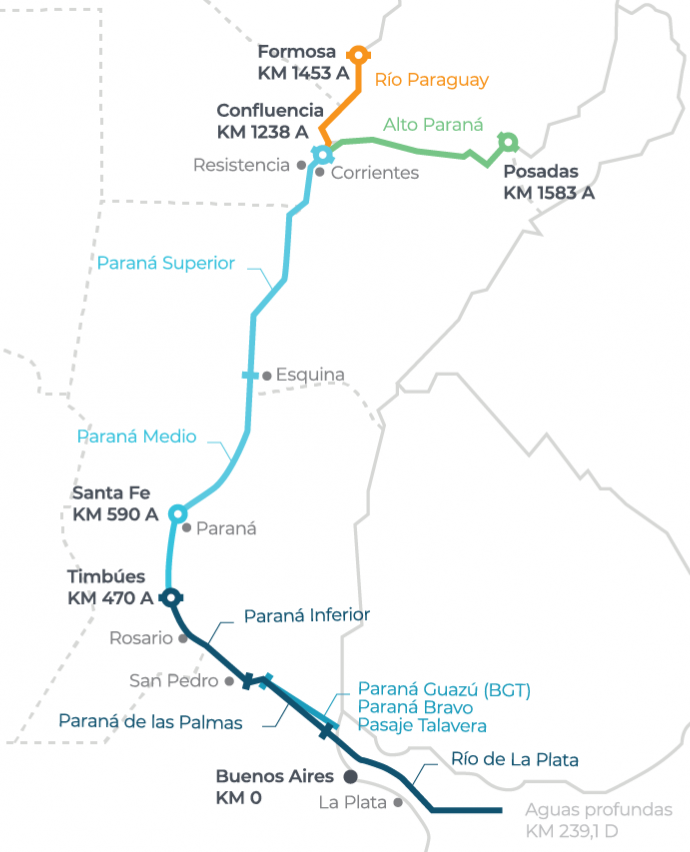
\includegraphics[width=0.5\linewidth]{figures/ch2/2025_mapa_vnt_extendida_tramos_profundidades_abril.png}
  %  \caption{The Vía Navegable Troncal (VNT) and the location of the Paraná and Paraná Guazú in it \autocite{agencianacionaldepuertosynavegacionNavegableTroncal2025}}
 %   \label{fig:VNT}
%\end{figure}

The Paraná River is formed by the junction of the rivers Grand and Paranaíba in south-central Brazil and flows for 4880 kilometers until it empties in the Río de la Plata near Buenos Aires, Argentina \autocite{orfeoHydraulicMorphologicalCharacteristics2002}. The river can be split up in three different sections: the upper, middle and lower Paraná. For these sections, the general characteristics related to discharge, channel size, and sediments are discussed.

The Upper Paraná River flows southwest, from the origin of the Paraná, until the confluence with the Paraguay river. Mean annual discharges at Porto São José, located near Porto Primavera at the confluence of the Paraná and Paranapanema in figure \ref{fig:rio parana map}, are between 6501 to 13,294 m³/s. The maximum flow velocity varies between 0.6–0.9 m/s in tributary channels and up to 1.4 m/s in the main channel during floods \autocite{stevauxUpperParanaRiver1994}. The Upper Paraná River exhibits a multi-channeled, braided pattern with numerous islands and sand bars, and its floodplain is strongly asymmetrical, being much wider on the right side (4.2–8.5 km) while the left margin erodes the Caiuá Formation \autocite{orfeoHydraulicMorphologicalCharacteristics2002}. During normal floods, water enters the floodplain through secondary and abandoned channels, producing slow and non-unidirectional flow, but extreme floods can cause crevasses and temporary channels. The channel is 1200–4500 m wide and 6–17 m deep with a slope of 0.096 m/km \autocite{stevauxUpperParanaRiver1994}. Finally, the suspended sediment concentration at Porto Rico, just South of Porto São José, equal 14.8×10⁶ tons/year and is mainly composed of quartz, mica, and kaolinite. The bed load at this location has a total discharge of 4.04×10⁶ tons/year and consists of quartz-rich (95\%) medium to fine sand \autocite{stevauxUpperParanaRiver1994}.

After the confluence with the Paraguay river, the Upper Paraná goes over into the Middle Paraná River. This part of the river stretches until the start of the delta, just South of Rosario City. Near Corrientes City, South of the confluence, the mean annual discharge is 16,941 m³/s, with summer floods (Feb–Mar) and spring low water levels, reaching maximum values above 50,000 m³/s. The channel width ranges 1.9–4.7 km, with depths of 15–20 m and a slope of 0.085 m/km \autocite{orfeoHydraulicMorphologicalCharacteristics2002}. Below the Paraguay River confluence, suspended sediment concentrations are highly variable due to differences in discharge, confluence angle, and sediment characteristics between both rivers. The suspended solid concentration ranges from 18 to 554 mg/l, with the right margin showing much higher values (up to 1221 mg/l) than the left (maximum 88 mg/l) (Bonetto & Orfeo, 1984). The suspended load is mainly silt (61–66\%) on the right margin and clay (79\%) on the left, with minor fine sand. The bed load is composed mostly of medium to fine quartz sand. The total sediment discharge is estimated at 158.4×10⁶ tons/year, with suspended load contributing 75\% of that.

The final and smallest part of the Paraná is the Paraná delta, that ranges for around 320 kilometers, from Diamante, Entre Ríos, until the Río de la Plata near Buenos Aires. It is divided into three large regions: the Upper delta (from Diamante to Villa Constitución, Santa Fe province), the Middle delta (from Villa Constitución to Puerto Ibicuy, Entre Ríos province) and the Lower delta (from Puerto Ibicuy to the mouth of estuary called Río de la Plata). As mentioned in the introduction, this study focuses on the Lower delta specifically. Just upstream of the delta apex, near the city of Paraná, the mean annual discharge is 18,500 m³/s with peak discharges up to 60,000 m³/s. 

Jaime, P., Menendez, A., 2002. Análisis del régimen hidrológico de los ríos Paraná y
Uruguay. Informe LHA 05-216-02, Proyecto LHA 216, Instituto Nacional de Agua
(INA), Buenos Aire

Its width varies between 18 and 60 kilometres. The Paraná delta is characterized by many islands, which exist due to the large amounts of sediment that the Paraná delta carries: at its mouth it transports approximately a total of 160,000,000 tons of sediments per year. The particle load distribution is as follows: 25\% consists of clay, 60\% is silt and around 15\% can be characterized as sand. This sediment is deposited in the joint Paraná and Uruguay estuary, the Río de la Plata https://academia-lab.com/encyclopedia/parana-delta/?utm_source=chatgpt.com. 


%\section{Classification of Rio Paraná}
%Rivers can be described and classified in different ways. This classification can be linked to several factors such as age, colour or seasonality. 

%\subsection{The Age Classification of a River}
%Based on the development of the channel stage of a river, it can be labeled as youthful, mature or old age.  \autocite{davisGeographicalCycle1899}
%Applying this to the Rio Paraná makes it a complicated choice since the river is so long that it possesses features linked to each age label at distinct locations. therefore, it would be wiser to divide the Rio Paraná in three parts: upper, middle and lower Paraná. A youthful channel can be recognized through rapid flow, significant erosion, and a steep gradient. All these traits can be attributed to the upper Paraná zone.
%Moving on, a mature channel stage of river is in most cases a developed floodplain in the form of loops, called 'meander', and lateral erosion. This is mostly what can be seen in the middle part of the Paraná river.
%Lastly, the characteristics of an old age channel are comparable to the lower Paraná river. A wider floodplain, less rapid flow, and deltas. All of this is explained in \cite{orfeoParanaRiverArgentine2023}, and can be seen in the following Figure \ref{fig:rio parana map} from \cite{lopezweibelSourcesTemporalDynamics2022}.

Upper, middle, lower
Chars of each section

\begin{figure}[H]
    \centering    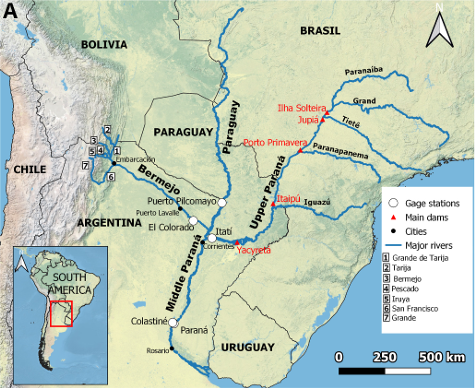
\includegraphics[width=0.7\linewidth]{figures/ch2/map rio parana.png}
    \caption{Rio Paraná Map}
    \label{fig:rio parana map}
\end{figure}


%From Davis's study it follows logically that all these stages are represented in the total picture of the Paraná river since it is the ninth largest river in the world based on discharge \autocite{lopezweibelSourcesTemporalDynamics2022}.

%\subsection{The Colour Classification of a River}
%The colour of the river is also another label that can create a distinction. Based on two sets of papers/research  \autocite{furchWaterChemistryAmazon1984}, \autocite{sioliAmazonLimnologyLandscape1984}  Junk 1997, the water in rivers can be described as black, white or clear. The black water river is attributed to the 'leaching of tannins from decayed leaves of adjoining vegetated lands' \autocite{sand-mining-boek}, most common in Amazonia or in the United States. White waters on the other hand are, contrary to its qualification, usually brown coloured due to the high sediment concentration. Clear water rivers are located in environments with little to no erosion.
%Based on the theory and satellite imagery, one can again classify the Rio Paraná in different as a black and white river depending on the zone. The upper Paraná can be considered to be black due to its lack of sediment content, but rich in leaves content. But after the Bermejo river joins the Paraná, the river turns muddy all the way to the sea near Buenos Aires, as seen in Figure \ref{fig:confluences} \autocite{lopezweibelSourcesTemporalDynamics2022}.

\begin{comment}
    \begin{figure}[H]
    \centering
    \begin{subfigure}[b]{0.48\textwidth}
        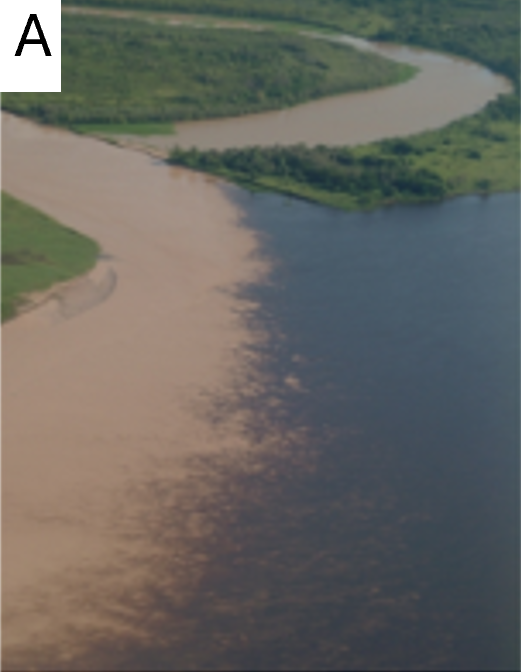
\includegraphics[width=\linewidth, height=5cm]{figures/ch2/Paraguay-Bermejo.png}
        \caption{Confluence of the Paraguay and Bermejo River}
        \label{fig:bermejo}
    \end{subfigure}
    \hfill
    \begin{subfigure}[b]{0.48\textwidth}
        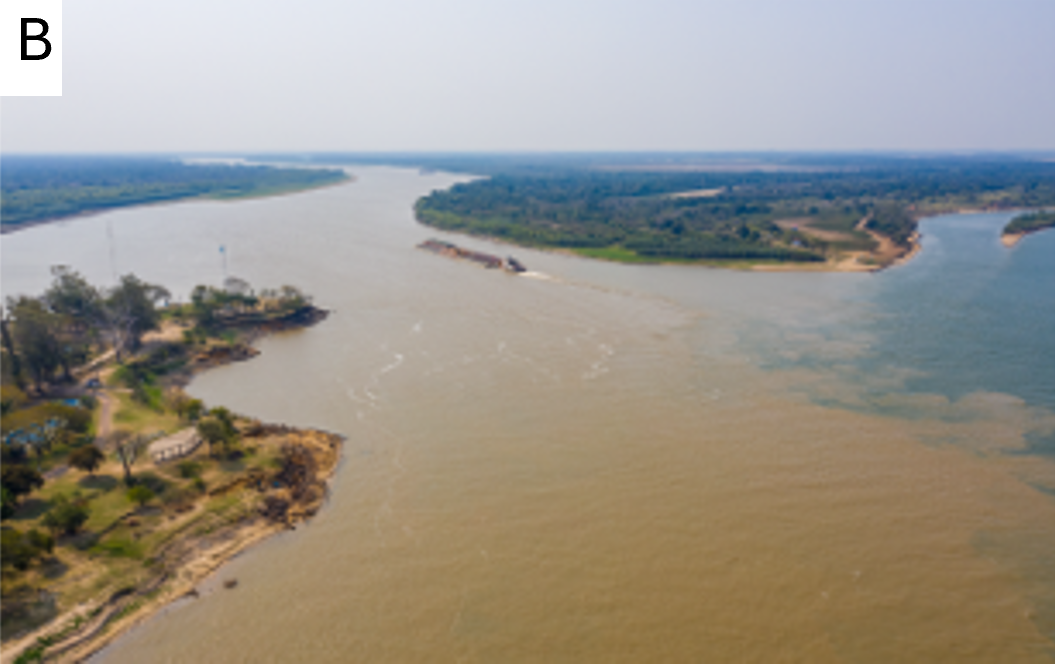
\includegraphics[width=\linewidth, height=5cm]{figures/ch2/Paraguay Parana.png}
        \caption{Confluence of the Paraguay and Paraná River}
        \label{fig:parana}
    \end{subfigure}
    \caption{Confluences of the Paraguay River with the Bermejo (left) and Paraná (right)}
    \label{fig:confluences}
    \end{figure}
\end{comment}


%\subsection{The Seasonal Flow of a River}
%The last classification relevant for this study is based on the flow characteristics and water availability. There are once again three types of categories: ephemeral, intermediate and perennial rivers. Ephemeral means that the river flow is not continuously present throughout the calendar year. Perennial rivers are the rivers whose flow is continuous and does not dry up during dry season, unlike the ephemeral rivers. Lastly the intermediate rivers are perennial rivers that dry up in extreme cases of drought.
%The Rio Paraná can be considered a perennial river due to its continuous flow over the years \autocite{furchWaterChemistryAmazon1984}, \autocite{sioliAmazonLimnologyLandscape1984}.

\section{Origin of sediment content in Paraná Guazú}
\label{sec:origin sediment content}

A key step in constructing the sediment balance of the Paraná Guazú, located in the lower Paraná, is to identify the origin of its sediment. As shown in Figure \ref{fig:placeholder}, the lower and middle Paraná receive discharge from three main tributaries: the Bermejo, Paraguay, and Upper Paraná Rivers. The total average discharge in the middle Paraná is $18,389~\mathrm{m^3/s}$, of which 78\% is supplied by the upper Paraná. \citeauthor{lopezweibelSourcesTemporalDynamics2022} report that the Bermejo contributes only 2\% of this discharge. Nevertheless, the Bermejo is the dominant source of sediment, due to intense erosion in the Andes Eastern Mountain Range within its basin. During the wet season (November to April), multiple tributaries in the basin contribute large sediment flows, accumulating to an annual suspended sediment load of $106 ~\times 10^6$ t per year at El Colorado gauge station. 

It is interesting to know that the contribution of sediment from the Bermejo to the Paraná is approximately 90\% today, but that this is in fact due to the installation of the Itaipu dam built in 1971, located in the south of Brazil just before the border with Argentina and Paraguay. This modification of the sediment voyage cuts a supply of about 50\% compared the initial amount of sediment, this 90\% used to be 56\% of the sediment income before the construction of the dam. This explains us that the human action already hindered the initial inflow of sediment a long time ago \autocite{hibaParanaRiverEcological2024}.

In summary, while the Paraguay and Upper Paraná Rivers provide most of the fluvial discharge to the downstream delta, the Bermejo River delivers the majority of sediments \autocite{lopezweibelSourcesTemporalDynamics2022}. For this reason, the stretch of river beginning in the Bermejo basin and continuing via the Paraguay and middle Paraná to the Paraná Guazú is of particular importance in this study.  

\section{Mining of the Sand and Types of Dredging in a River}
Due to the need of sand in human society, various techniques have been established to get hold of the sand in the river beds. For the sake of this study the focus lies on in-stream mining, the extraction of sand and gravel from the active channel of a river \autocite{sand-mining-boek}. The following types of in-stream dredging exist.

\textit{Bar scalping or skimming}:
This is the most common practice of extraction. It consists of taking away the two thirds of the bar, leaving the top third to minimize the alternation of the river bed initial conditions.

\textit{Dry pit channel mining}:
This method relies on using tools (mechanical or manual) to create a dry pit in which the sand or gravel can be extracted. The state in which the pits are left after extraction act has head cuts, altering the upstream flow during the high seasons.

\textit{Wet pit channel mining}:
Usually, the pit is made in a perennial river, but the effects and damages are the same as for the dry pit channel mining.

\textit{Bar excavation}:
This excavation process happens downstream of the bar, in order to get a hold of the sand and gravel going downstream.

\textit{Instream traps}:
For this excavation method a hole is dug so that the sediment gets caught during high season. This sediment can later be captured when the tides are low again.



\section{The effects of river sand mining}
\subsection{River bed}
As mentioned previously, rivers maintain an equilibrium between erosion, transport, and deposition of sediments. However, instream sand mining can discrupt this balance. This happens through direct disruption of the channel geometry or through so-called incision and related undercutting of banks \autocite{sand-mining-boek}.

The direct disruption of the river bed depends on the type of sand mining technique employed. In the case of pit excavation, the river bed is locally lowered and a so-called 'nick point' is created. With bar skimming the river bed is widened \autocite{sand-mining-boek}. For the remainder of this section, the consequent effects of the local river bed lowering (the nick point) are discussed.

Channel incision causes the nick point to migrate both upstream and downstream. In the case of high flows, due to its shape, the nick point is the point where most erosion occurs. Water plunges over the step and erodes the bed at the base. As flows continue, the drop migrates upstream, a process which is often called head-cutting in literature. On the other hand, a process called 'hungry water' causes downstream migration of the pit \autocite{sand-mining-boek}.

A the mining pit the water level is deeper, which causes the flow velocity to reduce locally. This leads to a decrease in flow energy and thus to more deposited sediment. When the flow leaves the mining area, water levels are shallower again meaning that flow velocity and energy significantly increase. A lot of sediment has been deposited in the nick point, meaning that the water is not using its full sediment carrying capacity anymore. In other words, the water is 'hungry' for sediment and erosion downstream increases \autocite{sand-mining-boek}. 

Through the combined effects of head-cutting and hungry water, the mining pit can extend beyond the initial dimensions caused by direct disruption. This happens in both downstream and upstream directions, as summarized in figure \ref{fig:channelbedeffects}.

\begin{figure}[H]
    \centering
    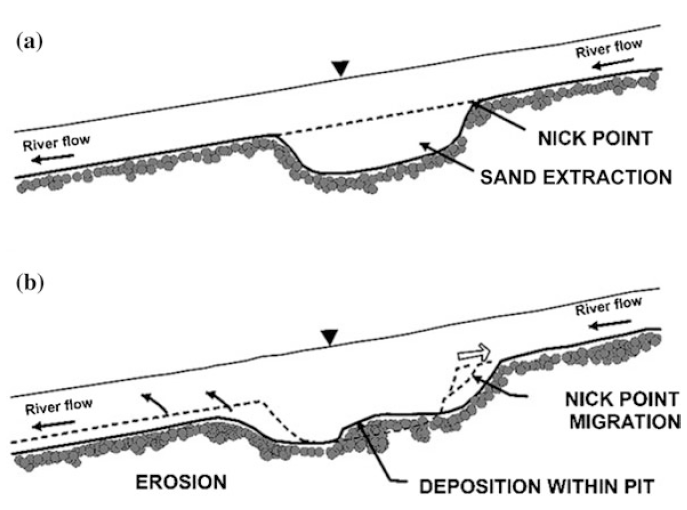
\includegraphics[width=0.75\linewidth]{figures/channelbedeffects.png}
    \caption{a: direct disruption leads to a locally lowered water bed, b: channel incision makes the pit migrate upstream through head cutting and downstream through 'hungry' water \autocite{sand-mining-boek}}
    \label{fig:channelbedeffects}
\end{figure}

\subsection{Sediment}
Previous studies have shown that bed coarsening can occur as a result of sand-mining. Fine particles are removed, leading to a greater concentration of coarse (gravelly) particles. This effect can also be seen upstream \autocite{sand-mining-boek}.

\subsection{Water quality and quantity}
Sand mining can lead to changes in both water quality and quantity. The process of dredging the fine sand stirs fine organic and inorganic particles, thereby increasing the turbidity of the water. This reduces light penetration, which means less photosynthesis and ultimately less organic growth in the water \autocite{sharipEffectsSeasonSand2014}.

As mentioned before, mining pits are often places with significant deposition of particles. Fine, nutrient-rich particles can settle and get trapped in the pits. This then reduces the transport of nutrients from the river to the coastal waters \autocite{sand-mining-boek}.

Concerning the water quantity, the most relevant effects are related to the groundwater: the lowering of the river bed through direct disruption or channel incision can lead to a lower groundwater table. This can lead to settlements or have negative effects on flora and fauna surrounding the river \autocite{rentierEnvironmentalImpactsRiver2022}.

\subsection{Biologic, socioeconomic and infrastructural changes}
The effects of sand mining can be diverse: previous studies have shown negative impacts on biodiversity, including reduced benthic fauna, disrupted fish spawning habitats, and depletion of natural mosquito predators such as dragonflies \autocite{sand-mining-boek}. The socioeconomic effects of mining can vary, in the short-term it often provides employment, income, and government revenue through royalties and taxation. However, in the long-term the operation can cause a reduction in access to clean water and can cause water scracity, especially in dry periods. Additionally, loss of land and access to land together with loss of trees and vegetation can jeopardize the local food security. Finally, infrastructure can be damaged by the lowering of the river bed and/or the groundwater table \autocite{sand-mining-boek}.